\documentclass[12pt]{article}
\usepackage{array}
\usepackage{color}
\usepackage{amsthm}
\usepackage{eufrak}
\usepackage{lipsum}
\usepackage{pifont}
\usepackage{yfonts}
\usepackage{amsmath}
\usepackage{amssymb}
\usepackage{ccfonts}
\usepackage{comment} \usepackage{amsfonts}
\usepackage{fancyhdr}
\usepackage{graphicx}
\usepackage{listings}
\usepackage{mathrsfs}
\usepackage{setspace}
\usepackage{textcomp}
\usepackage{blindtext}
\usepackage{enumerate}
\usepackage{microtype}
\usepackage{xfakebold}
\usepackage{kantlipsum}
%\usepackage{draftwatermark}
\usepackage[spanish]{babel}
\usepackage[margin=1.5cm, top=2cm, bottom=2cm]{geometry}
\usepackage[framemethod=tikz]{mdframed}
\usepackage[colorlinks=true,citecolor=blue,linkcolor=red,urlcolor=magenta]{hyperref}

%//////////////////////////////////////////////////////
% Watermark configuration
%//////////////////////////////////////////////////////
%\SetWatermarkScale{4}
%\SetWatermarkColor{black}
%\SetWatermarkLightness{0.95}
%\SetWatermarkText{\texttt{Watermark}}

%//////////////////////////////////////////////////////
% Frame configuration
%//////////////////////////////////////////////////////
\newmdenv[tikzsetting={draw=gray,fill=white,fill opacity=0},backgroundcolor=none]{Frame}

%//////////////////////////////////////////////////////
% Font style configuration
%//////////////////////////////////////////////////////
\renewcommand{\familydefault}{\ttdefault}
\renewcommand{\rmdefault}{tt}

%//////////////////////////////////////////////////////
% Bold configuration
%//////////////////////////////////////////////////////
\newcommand{\fbseries}{\unskip\setBold\aftergroup\unsetBold\aftergroup\ignorespaces}
\makeatletter
\newcommand{\setBoldness}[1]{\def\fake@bold{#1}}
\makeatother

%//////////////////////////////////////////////////////
% Default font configuration
%//////////////////////////////////////////////////////
\DeclareFontFamily{\encodingdefault}{\ttdefault}{%
  \hyphenchar\font=\defaulthyphenchar
  \fontdimen2\font=0.33333em
  \fontdimen3\font=0.16667em
  \fontdimen4\font=0.11111em
  \fontdimen7\font=0.11111em}



\begin{document}
    %//////////////////////////////////////////////////////
% Heading Configuration
%//////////////////////////////////////////////////////
\pagestyle{fancy}
\thispagestyle{plain}
\fancyhead[RO,L]{\textbf{Teoria de Grafos}}
\fancyhead[LO,L]{\textbf{Tarea 2}}
\setlength{\headheight}{16.0pt}

%//////////////////////////////////////////////////////
% Subsections Configuration
%//////////////////////////////////////////////////////
\renewcommand*\thesubsection{\arabic{subsection}}
\newcounter{counter}
\newlength{\palabra}
\settowidth{\palabra}{counter 999.}
\newcommand{\makeboxlabel}[1]{\fbox{#1.}\hfill}

%//////////////////////////////////////////////////////
% Personalized commands configuration
%//////////////////////////////////////////////////////
\newcommand{\N}{\mathbb{N}}
\newcommand{\Z}{\mathbb{Z}}
\newcommand{\Q}{\mathbb{Q}}
\newcommand{\R}{\mathbb{R}}
\newcommand{\C}{\mathbb{C}}
\newcommand{\re}{\operatorname{Re}}
\newcommand{\im}{\operatorname{Im}}
\newcommand{\Aut}{\operatorname{Aut}}
\newcommand{\GCD}{\operatorname{GCD}}
\newcommand{\LCD}{\operatorname{LCD}}
\linespread{1} %Line spacing

%//////////////////////////////////////////////////////
% Inline code configuration
%//////////////////////////////////////////////////////
\lstset{
gobble=5,
numbers=left,
frame=single,
framerule=1pt,
showtabs=False,
showspaces=False,
showstringspaces=False,
backgroundcolor=\color{gray}}

%//////////////////////////////////////////////////////
% Problem list configuration
%//////////////////////////////////////////////////////
\newenvironment{problems}
  {\begin{list}
     {{\fbseries Problem \arabic{counter}.}}
    {\usecounter{counter}
     \setlength{\labelsep}{1em}
     \setlength{\itemsep}{2pt}
     \setlength{\leftmargin}{2em}
     \setlength{\rightmargin}{0cm}
     \setlength{\itemindent}{1em} }}
{\end{list}}

%//////////////////////////////////////////////////////
% Appendix configuration
%//////////////////////////////////////////////////////
\newenvironment{Appendix}
  {\begin{list}
     {{\fbseries Lemma \arabic{counter}.}}
    {\usecounter{counter}
     \setlength{\labelsep}{1em}
     \setlength{\itemsep}{2pt}
     \setlength{\leftmargin}{2em}
     \setlength{\rightmargin}{0cm}
     \setlength{\itemindent}{1em} }}
{\end{list}}

%//////////////////////////////////////////////////////
% Notes configuration
%//////////////////////////////////////////////////////
\newenvironment{notes}
  {\begin{list}
     {{\fbseries Note \arabic{counter}.}}
    {\usecounter{counter}
     \setlength{\labelsep}{1em}
     \setlength{\itemsep}{2pt}
     \setlength{\leftmargin}{2em}
     \setlength{\rightmargin}{0cm}
     \setlength{\itemindent}{1em} }}
{\end{list}}

%//////////////////////////////////////////////////////
% Activity Information
%//////////////////////////////////////////////////////
\vspace*{-1cm}
\hrule width \hsize \kern 1mm \hrule width \hsize height 2pt
\begin{center}
   \parbox[c]{.32\textwidth}{
   \hspace{1cm}\\
   Sergio Montoya Ramirez\\
   202112171}
%   Luis Ernesto Tejón Rojas\\
%   202113150}
   \hspace*{\fill}
   \parbox[c]{.35\textwidth}{\centering
   Universidad de Los Andes\\
   Tarea 1\\
   Teoria de Grafos\\
   }
   \hspace*{\fill}
   \parbox[c]{.3\textwidth}{
   \begin{flushleft}
      Bogotá D.C., Colombia\\
      \today
   \end{flushleft}}
\end{center}
\hrule width \hsize height 2pt \kern 1mm \hrule width \hsize

\bigskip

\bigskip


    \section*{Primera Pregunta}

    Suponga por contradicción que $G$ es disconexo. Dado que $d_x, d_y > 0$ entonces estas componentes deben estar repartidas entre $X$ y $Y$. Ahora bien, sabemos por la clase que el numero de arcos de una componente conexa de $m$ elementos es al menos $m-1$. Sin embargo, en este caso dado que tenemos que el mínimo valor que puede tomar la suma del grado de dos vértices es $\frac{n}{2}$ estas componentes superarían lo que esperábamos y en consecuencia debería ser conexo.

    \section*{Segunda Pregunta}

    \subsection*{General}

    Dado que $L\left( G \right) = K_n$ sabemos que $G$ tiene $n$ arcos.
    
    \subsection*{Primera Parte}

    Dado que $n\neq 3$ entonces estos vértices tienen asociados mas de dos arcos. Ahora bien, con esto podemos organizar los arcos de cada vértice en $L\left( G \right) $ de tal forma que todo salga de un mismo punto por lo que es isomorfo a $S_n$

    \subsection*{Segunda Parte}

    En el caso de $n=3$ existen 2 posibilidades.
     \begin{enumerate}
      \item Cada vértice tiene exactamente dos arcos conectados directamente a un vértice. En donde este seria isomorfo a $S_3$ 
      \item Uno de los vértices tiene 3 arcos y los otros dos tienen 2. En cuyo caso esto equivale a $K_3$
    \end{enumerate}


    
    \section*{Tercera Pregunta}

    El árbol recubridor mínimo seria:

    \begin{figure}[H]
      \centering
      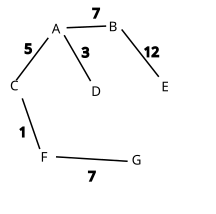
\includegraphics[width=0.4\textwidth]{Imagenes/grafo1.png}
      \caption{Árbol recubridor mínimo del grafo puesto en el punto 3 de la tercera tarea}
      \label{fig:grafo1}
    \end{figure}

    Y el orden en el que entraron los vértices fue:
    \begin{enumerate}
      \item $\left\{ C, F \right\} $ 
      \item $\left\{ A,D \right\} $ 
      \item $\left\{ A,C \right\} $ 
      \item $\left\{ A,B \right\} $ 
      \item $\left\{ F,G \right\} $ 
      \item $\left\{ B,E \right\} $
    \end{enumerate}

    \section*{Cuarta Pregunta}
    \subsection*{Primera Parte}

    Asuma por contradicción que existe un árbol recubridor tal que este no comparta ningún vértice con $E$. Por lo tanto todos sus vértices se encuentran en $G-S$. Sin embargo, dado que $E$ es un \textit{Edge-cut} sabemos que  $G-S$ es disconexo y por lo tanto contradictorio.

    \subsection*{Segunda Parte}

    En este caso aprovecharemos la segunda característica. En particular tomo como contraejemplo:
    \begin{figure}[H]
      \centering
      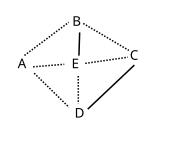
\includegraphics[width=0.4\textwidth]{Imagenes/grafo2}
      \caption{Grafo contra ejemplo}
      \label{fig:grafo2}
    \end{figure}

    En este caso si bien es cierto que el conjunto $G-E$ es disco nexo también se da que no puede existir un $S$ tal que $E = [S,\overline{S}]$

    \section*{Nota}

    Para la realización de este taller se converso con 3 compañeros en la solución de Dudas:
    \begin{enumerate}
      \item Ángel
      \item Germán López
      \item Gabriela
    \end{enumerate}
\end{document}
